% Add \usepackage{graphicx,amsmath,amssymb} to the manuscript preamble.
% Place this figures/ directory beside the manuscript and use:
% % Add \usepackage{graphicx,amsmath,amssymb} to the manuscript preamble.
% Place this figures/ directory beside the manuscript and use:
% % Add \usepackage{graphicx,amsmath,amssymb} to the manuscript preamble.
% Place this figures/ directory beside the manuscript and use:
% % Add \usepackage{graphicx,amsmath,amssymb} to the manuscript preamble.
% Place this figures/ directory beside the manuscript and use:
% \input{figures/model_architecture.tex}
% Use figure instead of figure* for a single-column manuscript.
% The original PDF is 180 x 140 mm. Use the vector PDF in the submission.
\begin{figure*}[t]
  \centering
  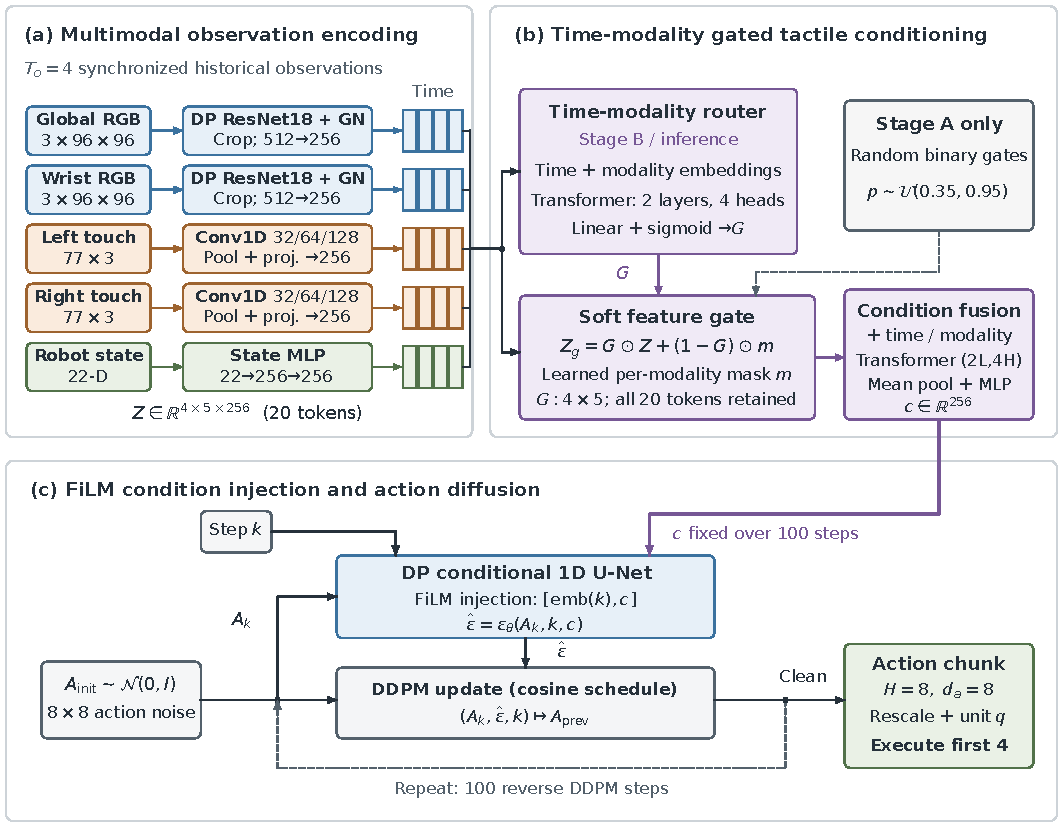
\includegraphics[width=\textwidth]{figures/model_architecture.pdf}
  \caption{TacGate-DP: time--modality gated tactile conditioning for diffusion policies.
  (a) Four synchronized historical observations are processed by five
  independent encoders: two Diffusion Policy (DP) ResNet18 visual encoders
  with GroupNorm, two one-dimensional tactile CNNs over taxel indices,
  and a robot-state MLP. Each tactile CNN uses channels 32, 64, and 128,
  followed by global average pooling and a 256-dimensional projection.
  Each time--modality pair yields a 256-dimensional
  token, forming $Z\in\mathbb{R}^{4\times5\times256}$.
  (b) An observation-only Transformer router predicts independent sigmoid
  gates $G\in[0,1]^{4\times5}$. Soft gating blends each observation token
  with a learned per-modality mask token $m$; all 20 token positions are
  retained. A separate Transformer with its own learned temporal and
  modality embeddings, followed by mean pooling and projection, produces
  the global condition $c\in\mathbb{R}^{256}$. Left and right tactile features
  thus enter action generation through gated, fused multimodal conditioning.
  (c) The fused condition, including tactile information, is injected into
  a DP conditional 1D U-Net through FiLM together with the diffusion-step
  embedding. The U-Net predicts action noise. The condition is computed once
  per action chunk and reused throughout 100 reverse DDPM steps. The final
  actions are rescaled and their quaternions normalized; the first four
  actions of the eight-step prediction are executed before replanning.
  Stage A substitutes random binary gates for the router output (dashed
  path); Stage B and inference use learned gates. The supplied Stage B
  configuration freezes the observation encoders. Batch dimensions are
  omitted; dimensions shown are the release defaults.}
  \label{fig:tacgate-dp}
\end{figure*}

% Use figure instead of figure* for a single-column manuscript.
% The original PDF is 180 x 140 mm. Use the vector PDF in the submission.
\begin{figure*}[t]
  \centering
  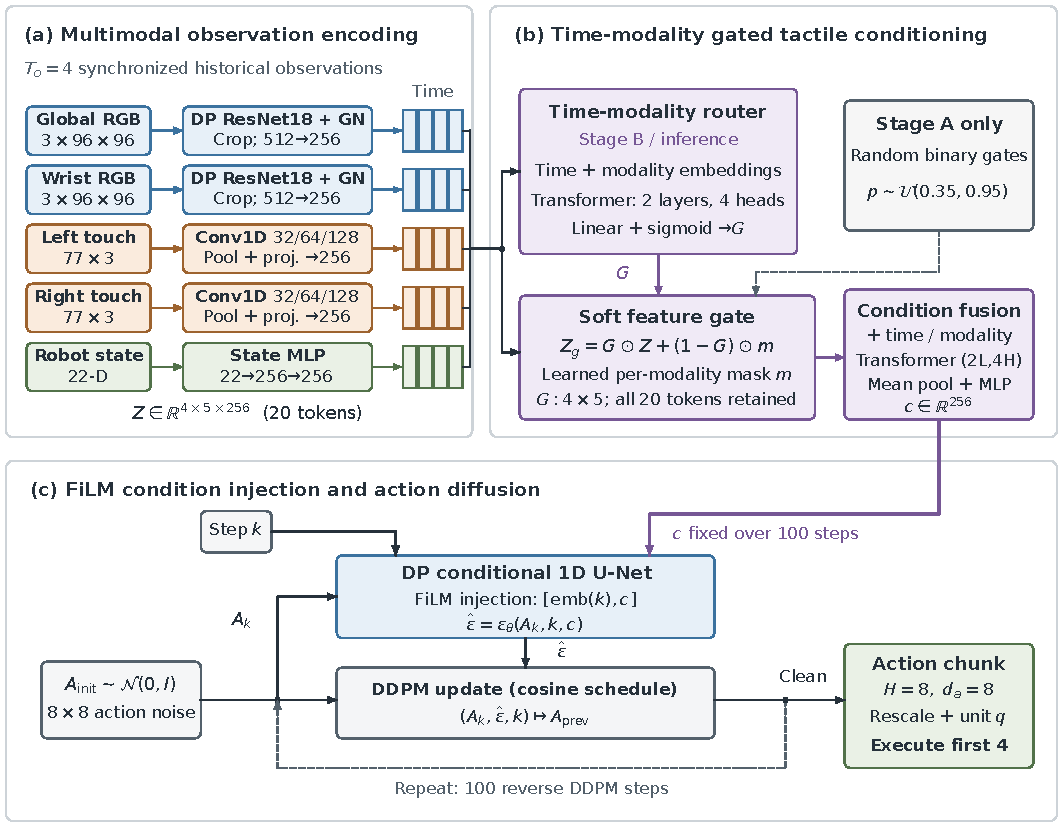
\includegraphics[width=\textwidth]{figures/model_architecture.pdf}
  \caption{TacGate-DP: time--modality gated tactile conditioning for diffusion policies.
  (a) Four synchronized historical observations are processed by five
  independent encoders: two Diffusion Policy (DP) ResNet18 visual encoders
  with GroupNorm, two one-dimensional tactile CNNs over taxel indices,
  and a robot-state MLP. Each tactile CNN uses channels 32, 64, and 128,
  followed by global average pooling and a 256-dimensional projection.
  Each time--modality pair yields a 256-dimensional
  token, forming $Z\in\mathbb{R}^{4\times5\times256}$.
  (b) An observation-only Transformer router predicts independent sigmoid
  gates $G\in[0,1]^{4\times5}$. Soft gating blends each observation token
  with a learned per-modality mask token $m$; all 20 token positions are
  retained. A separate Transformer with its own learned temporal and
  modality embeddings, followed by mean pooling and projection, produces
  the global condition $c\in\mathbb{R}^{256}$. Left and right tactile features
  thus enter action generation through gated, fused multimodal conditioning.
  (c) The fused condition, including tactile information, is injected into
  a DP conditional 1D U-Net through FiLM together with the diffusion-step
  embedding. The U-Net predicts action noise. The condition is computed once
  per action chunk and reused throughout 100 reverse DDPM steps. The final
  actions are rescaled and their quaternions normalized; the first four
  actions of the eight-step prediction are executed before replanning.
  Stage A substitutes random binary gates for the router output (dashed
  path); Stage B and inference use learned gates. The supplied Stage B
  configuration freezes the observation encoders. Batch dimensions are
  omitted; dimensions shown are the release defaults.}
  \label{fig:tacgate-dp}
\end{figure*}

% Use figure instead of figure* for a single-column manuscript.
% The original PDF is 180 x 140 mm. Use the vector PDF in the submission.
\begin{figure*}[t]
  \centering
  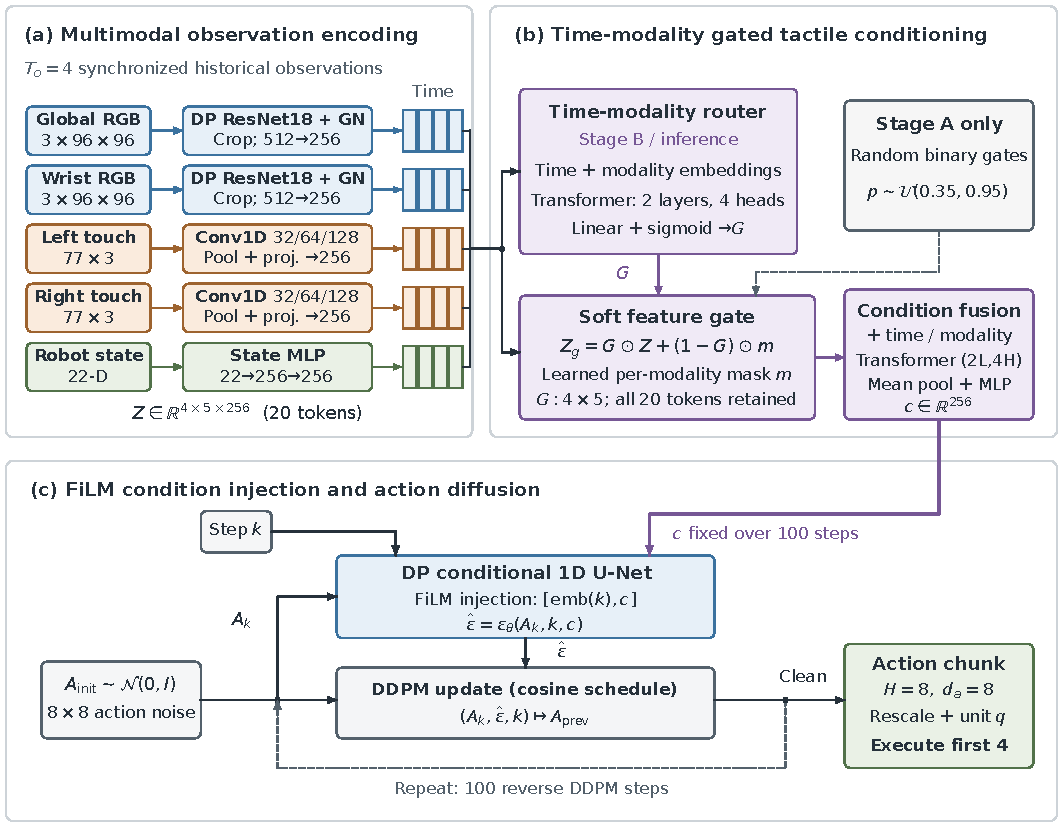
\includegraphics[width=\textwidth]{figures/model_architecture.pdf}
  \caption{TacGate-DP: time--modality gated tactile conditioning for diffusion policies.
  (a) Four synchronized historical observations are processed by five
  independent encoders: two Diffusion Policy (DP) ResNet18 visual encoders
  with GroupNorm, two one-dimensional tactile CNNs over taxel indices,
  and a robot-state MLP. Each tactile CNN uses channels 32, 64, and 128,
  followed by global average pooling and a 256-dimensional projection.
  Each time--modality pair yields a 256-dimensional
  token, forming $Z\in\mathbb{R}^{4\times5\times256}$.
  (b) An observation-only Transformer router predicts independent sigmoid
  gates $G\in[0,1]^{4\times5}$. Soft gating blends each observation token
  with a learned per-modality mask token $m$; all 20 token positions are
  retained. A separate Transformer with its own learned temporal and
  modality embeddings, followed by mean pooling and projection, produces
  the global condition $c\in\mathbb{R}^{256}$. Left and right tactile features
  thus enter action generation through gated, fused multimodal conditioning.
  (c) The fused condition, including tactile information, is injected into
  a DP conditional 1D U-Net through FiLM together with the diffusion-step
  embedding. The U-Net predicts action noise. The condition is computed once
  per action chunk and reused throughout 100 reverse DDPM steps. The final
  actions are rescaled and their quaternions normalized; the first four
  actions of the eight-step prediction are executed before replanning.
  Stage A substitutes random binary gates for the router output (dashed
  path); Stage B and inference use learned gates. The supplied Stage B
  configuration freezes the observation encoders. Batch dimensions are
  omitted; dimensions shown are the release defaults.}
  \label{fig:tacgate-dp}
\end{figure*}

% Use figure instead of figure* for a single-column manuscript.
% The original PDF is 180 x 140 mm. Use the vector PDF in the submission.
\begin{figure*}[t]
  \centering
  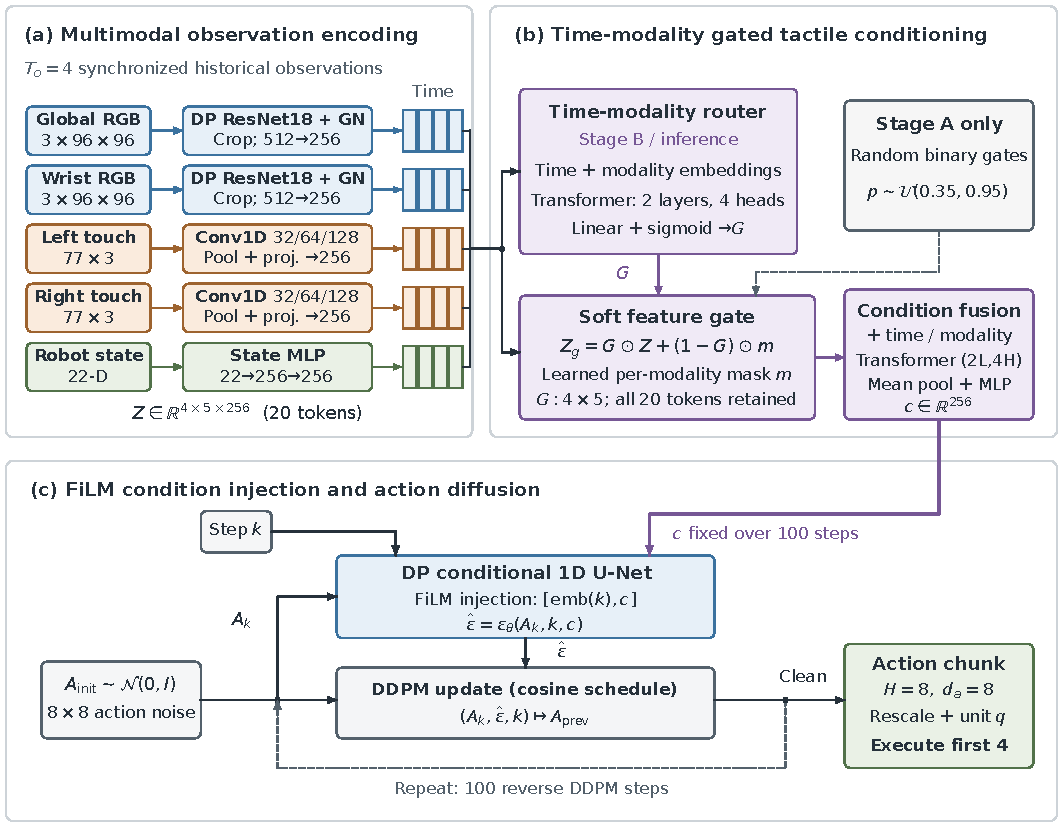
\includegraphics[width=\textwidth]{figures/model_architecture.pdf}
  \caption{TacGate-DP: time--modality gated tactile conditioning for diffusion policies.
  (a) Four synchronized historical observations are processed by five
  independent encoders: two Diffusion Policy (DP) ResNet18 visual encoders
  with GroupNorm, two one-dimensional tactile CNNs over taxel indices,
  and a robot-state MLP. Each tactile CNN uses channels 32, 64, and 128,
  followed by global average pooling and a 256-dimensional projection.
  Each time--modality pair yields a 256-dimensional
  token, forming $Z\in\mathbb{R}^{4\times5\times256}$.
  (b) An observation-only Transformer router predicts independent sigmoid
  gates $G\in[0,1]^{4\times5}$. Soft gating blends each observation token
  with a learned per-modality mask token $m$; all 20 token positions are
  retained. A separate Transformer with its own learned temporal and
  modality embeddings, followed by mean pooling and projection, produces
  the global condition $c\in\mathbb{R}^{256}$. Left and right tactile features
  thus enter action generation through gated, fused multimodal conditioning.
  (c) The fused condition, including tactile information, is injected into
  a DP conditional 1D U-Net through FiLM together with the diffusion-step
  embedding. The U-Net predicts action noise. The condition is computed once
  per action chunk and reused throughout 100 reverse DDPM steps. The final
  actions are rescaled and their quaternions normalized; the first four
  actions of the eight-step prediction are executed before replanning.
  Stage A substitutes random binary gates for the router output (dashed
  path); Stage B and inference use learned gates. The supplied Stage B
  configuration freezes the observation encoders. Batch dimensions are
  omitted; dimensions shown are the release defaults.}
  \label{fig:tacgate-dp}
\end{figure*}
